\documentclass{standalone}
\usepackage{tikz}
\usetikzlibrary{patterns, positioning}

\begin{document}
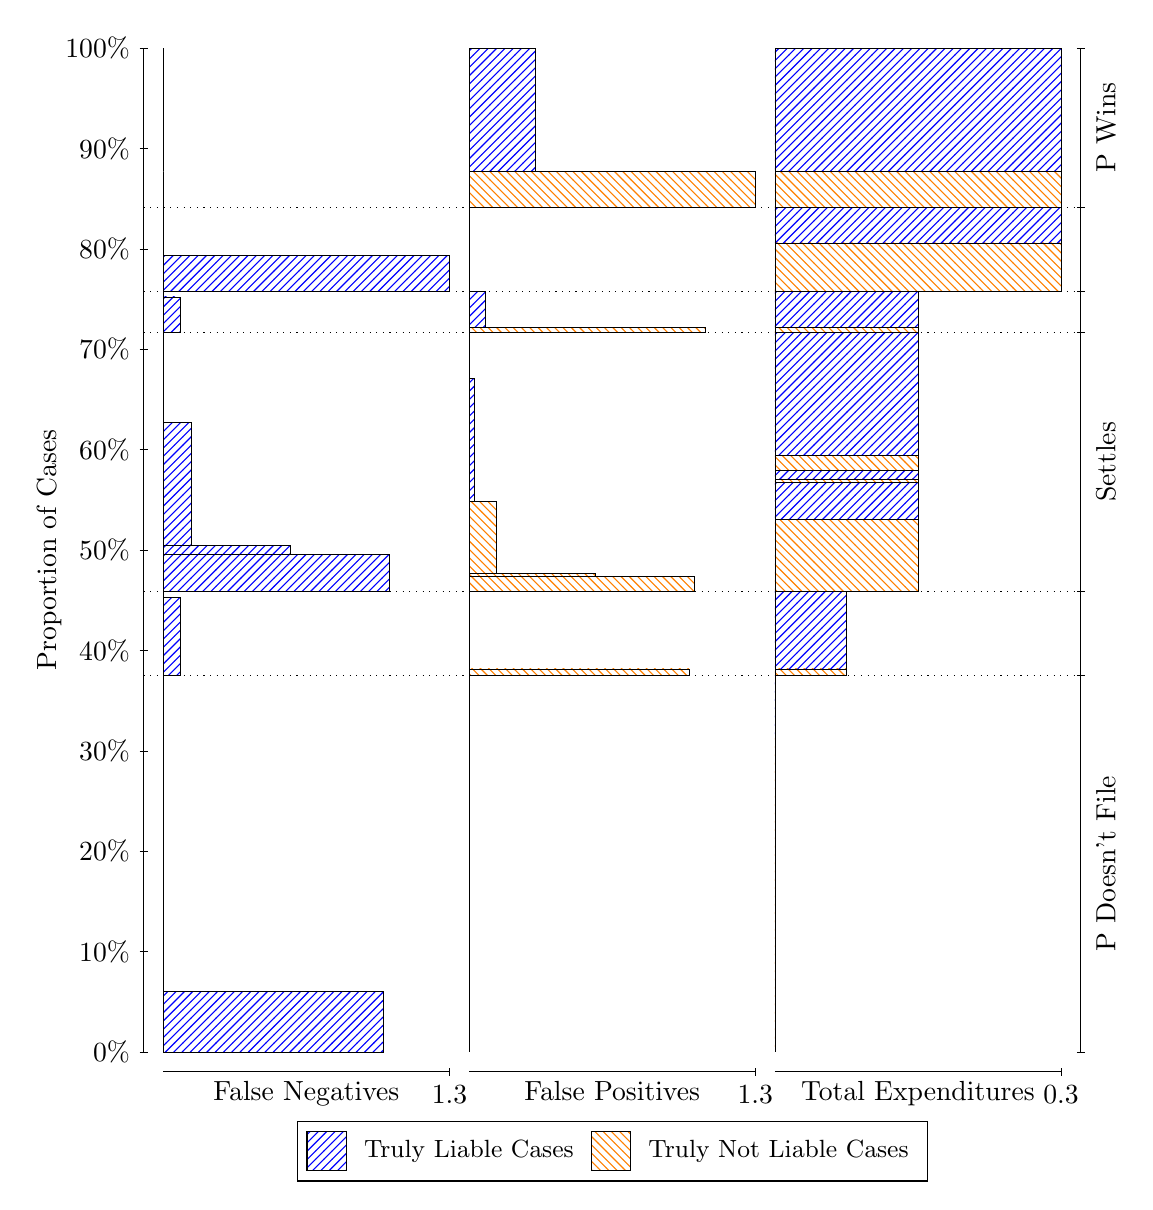
\begin{tikzpicture}
\draw[black, very thin] (1.5,1.75) -- (1.5,14.5);
\node[rotate=90, anchor=center] at (0.3, 8.125) {Proportion of Cases};
\draw[black, very thin] (1.45,1.75) -- (1.55,1.75);
\node[anchor=east] at (1.45, 1.75) {0\%};
\draw[black, very thin] (1.45,3.025) -- (1.55,3.025);
\node[anchor=east] at (1.45, 3.025) {10\%};
\draw[black, very thin] (1.45,4.3) -- (1.55,4.3);
\node[anchor=east] at (1.45, 4.3) {20\%};
\draw[black, very thin] (1.45,5.575) -- (1.55,5.575);
\node[anchor=east] at (1.45, 5.575) {30\%};
\draw[black, very thin] (1.45,6.85) -- (1.55,6.85);
\node[anchor=east] at (1.45, 6.85) {40\%};
\draw[black, very thin] (1.45,8.125) -- (1.55,8.125);
\node[anchor=east] at (1.45, 8.125) {50\%};
\draw[black, very thin] (1.45,9.4) -- (1.55,9.4);
\node[anchor=east] at (1.45, 9.4) {60\%};
\draw[black, very thin] (1.45,10.675) -- (1.55,10.675);
\node[anchor=east] at (1.45, 10.675) {70\%};
\draw[black, very thin] (1.45,11.95) -- (1.55,11.95);
\node[anchor=east] at (1.45, 11.95) {80\%};
\draw[black, very thin] (1.45,13.225) -- (1.55,13.225);
\node[anchor=east] at (1.45, 13.225) {90\%};
\draw[black, very thin] (1.45,14.5) -- (1.55,14.5);
\node[anchor=east] at (1.45, 14.5) {100\%};

\draw[black, very thin] (13.4,1.75) -- (13.4,14.5);
\draw[black, very thin] (13.35,1.75) -- (13.45,1.75);
\node[anchor=west] at (13.35, 1.75) {};
\draw[black, very thin] (13.35,6.5343) -- (13.45,6.5343);
\node[anchor=west] at (13.35, 6.5343) {};
\draw[black, very thin] (13.35,7.6024) -- (13.45,7.6024);
\node[anchor=west] at (13.35, 7.6024) {};
\draw[black, very thin] (13.35,10.886) -- (13.45,10.886);
\node[anchor=west] at (13.35, 10.886) {};
\draw[black, very thin] (13.35,11.407) -- (13.45,11.407);
\node[anchor=west] at (13.35, 11.407) {};
\draw[black, very thin] (13.35,12.48) -- (13.45,12.48);
\node[anchor=west] at (13.35, 12.48) {};
\draw[black, very thin] (13.35,14.5) -- (13.45,14.5);
\node[anchor=west] at (13.35, 14.5) {};

\draw[black, very thin, pattern color=blue, pattern=north east lines] (1.75,1.75) rectangle (4.5449,2.5199);
\draw[black, very thin, pattern color=orange, pattern=north west lines] (1.75,2.5199) rectangle (1.75,6.5343);
\draw[black, very thin, pattern color=blue, pattern=north east lines] (1.75,6.5343) rectangle (1.9596,7.5223);
\draw[black, very thin, pattern color=orange, pattern=north west lines] (1.75,7.5223) rectangle (1.75,7.6024);
\draw[black, very thin, pattern color=blue, pattern=north east lines] (1.75,7.6024) rectangle (4.6147,8.0715);
\draw[black, very thin, pattern color=blue, pattern=north east lines] (1.75,8.0715) rectangle (3.3571,8.1825);
\draw[black, very thin, pattern color=blue, pattern=north east lines] (1.75,8.1825) rectangle (2.0994,9.745);
\draw[black, very thin, pattern color=orange, pattern=north west lines] (1.75,9.745) rectangle (1.75,10.886);
\draw[black, very thin, pattern color=blue, pattern=north east lines] (1.75,10.886) rectangle (1.9596,11.34);
\draw[black, very thin, pattern color=orange, pattern=north west lines] (1.75,11.34) rectangle (1.75,11.407);
\draw[black, very thin, pattern color=blue, pattern=north east lines] (1.75,11.407) rectangle (5.3833,11.862);
\draw[black, very thin, pattern color=orange, pattern=north west lines] (1.75,11.862) rectangle (1.75,12.48);
\draw[black, very thin, pattern color=orange, pattern=north west lines] (1.75,12.48) rectangle (1.75,12.934);
\draw[black, very thin, pattern color=blue, pattern=north east lines] (1.75,12.934) rectangle (1.75,14.5);
\draw[black, very thin, pattern color=orange, pattern=north west lines] (5.6333,1.75) rectangle (5.6333,5.7644);
\draw[black, very thin, pattern color=blue, pattern=north east lines] (5.6333,5.7644) rectangle (5.6333,6.5343);
\draw[black, very thin, pattern color=orange, pattern=north west lines] (5.6333,6.5343) rectangle (8.4282,6.6143);
\draw[black, very thin, pattern color=blue, pattern=north east lines] (5.6333,6.6143) rectangle (5.6333,7.6024);
\draw[black, very thin, pattern color=orange, pattern=north west lines] (5.6333,7.6024) rectangle (8.4981,7.7872);
\draw[black, very thin, pattern color=orange, pattern=north west lines] (5.6333,7.7872) rectangle (7.2404,7.8293);
\draw[black, very thin, pattern color=orange, pattern=north west lines] (5.6333,7.8293) rectangle (5.9827,8.7432);
\draw[black, very thin, pattern color=blue, pattern=north east lines] (5.6333,8.7432) rectangle (5.7032,10.306);
\draw[black, very thin, pattern color=blue, pattern=north east lines] (5.6333,10.306) rectangle (5.6333,10.886);
\draw[black, very thin, pattern color=orange, pattern=north west lines] (5.6333,10.886) rectangle (8.6378,10.954);
\draw[black, very thin, pattern color=blue, pattern=north east lines] (5.6333,10.954) rectangle (5.8429,11.407);
\draw[black, very thin, pattern color=orange, pattern=north west lines] (5.6333,11.407) rectangle (5.6333,12.026);
\draw[black, very thin, pattern color=blue, pattern=north east lines] (5.6333,12.026) rectangle (5.6333,12.48);
\draw[black, very thin, pattern color=orange, pattern=north west lines] (5.6333,12.48) rectangle (9.2667,12.934);
\draw[black, very thin, pattern color=blue, pattern=north east lines] (5.6333,12.934) rectangle (6.4718,14.5);
\draw[black, very thin, pattern color=orange, pattern=north west lines] (9.5167,1.75) rectangle (9.5167,5.7644);
\draw[black, very thin, pattern color=blue, pattern=north east lines] (9.5167,5.7644) rectangle (9.5167,6.5343);
\draw[black, very thin, pattern color=orange, pattern=north west lines] (9.5167,6.5343) rectangle (10.425,6.6143);
\draw[black, very thin, pattern color=blue, pattern=north east lines] (9.5167,6.6143) rectangle (10.425,7.6024);
\draw[black, very thin, pattern color=orange, pattern=north west lines] (9.5167,7.6024) rectangle (11.333,8.5163);
\draw[black, very thin, pattern color=blue, pattern=north east lines] (9.5167,8.5163) rectangle (11.333,8.9854);
\draw[black, very thin, pattern color=orange, pattern=north west lines] (9.5167,8.9854) rectangle (11.333,9.0275);
\draw[black, very thin, pattern color=blue, pattern=north east lines] (9.5167,9.0275) rectangle (11.333,9.1385);
\draw[black, very thin, pattern color=orange, pattern=north west lines] (9.5167,9.1385) rectangle (11.333,9.3233);
\draw[black, very thin, pattern color=blue, pattern=north east lines] (9.5167,9.3233) rectangle (11.333,10.886);
\draw[black, very thin, pattern color=orange, pattern=north west lines] (9.5167,10.886) rectangle (11.333,10.954);
\draw[black, very thin, pattern color=blue, pattern=north east lines] (9.5167,10.954) rectangle (11.333,11.407);
\draw[black, very thin, pattern color=orange, pattern=north west lines] (9.5167,11.407) rectangle (13.15,12.026);
\draw[black, very thin, pattern color=blue, pattern=north east lines] (9.5167,12.026) rectangle (13.15,12.48);
\draw[black, very thin, pattern color=orange, pattern=north west lines] (9.5167,12.48) rectangle (13.15,12.934);
\draw[black, very thin, pattern color=blue, pattern=north east lines] (9.5167,12.934) rectangle (13.15,14.5);
\draw[black, dotted] (1.5,6.5343) -- (13.4,6.5343);
\draw[black, dotted] (1.5,7.6024) -- (13.4,7.6024);
\draw[black, dotted] (1.5,10.886) -- (13.4,10.886);
\draw[black, dotted] (1.5,11.407) -- (13.4,11.407);
\draw[black, dotted] (1.5,12.48) -- (13.4,12.48);
\draw[black, very thin] (1.75,1.5) -- (5.3833,1.5);
\node[anchor=north] at (3.5667, 1.5) {False Negatives};
\draw[black, very thin] (5.3833,1.45) -- (5.3833,1.55);
\node[anchor=north] at (5.3833, 1.45) {1.3};

\draw[black, very thin] (5.6333,1.5) -- (9.2667,1.5);
\node[anchor=north] at (7.45, 1.5) {False Positives};
\draw[black, very thin] (9.2667,1.45) -- (9.2667,1.55);
\node[anchor=north] at (9.2667, 1.45) {1.3};

\draw[black, very thin] (9.5167,1.5) -- (13.15,1.5);
\node[anchor=north] at (11.333, 1.5) {Total Expenditures};
\draw[black, very thin] (13.15,1.45) -- (13.15,1.55);
\node[anchor=north] at (13.15, 1.45) {0.3};

\node[black, centered, rotate=90] at (13.72, 4.1421) {P Doesn't File};

\node[black, centered, rotate=90] at (13.72, 9.2441) {Settles};


\node[black, centered, rotate=90] at (13.72, 13.49) {P Wins};

\draw (7.449999999999999,1.5) node[draw=none] (baseCoordinate) {};
\begin{scope}[align=center]
        \matrix[scale=0.5, draw=black, below=0.5cm of baseCoordinate, nodes={draw}, column sep=0.1cm]{
            \node[rectangle, draw, minimum width=0.5cm, minimum height=0.5cm, pattern=north east lines, pattern color=blue] {}; &
            \node[draw=none, font=\small] (B) {Truly Liable Cases}; &
            \node[rectangle, draw, minimum width=0.5cm, minimum height=0.5cm, pattern=north west lines, pattern color=orange] {}; &
            \node[draw=none, font=\small] (B) {Truly Not Liable Cases}; \\
            };
\end{scope}

\end{tikzpicture}
\end{document}